La aplicación sigue una arquitectura por capas, añadiendo el patrón \textquote{Façade} para la comunicación entre capas.
El objetivo de dicha arquitectura es facilitar el desarrollo, mantenimiento y escalabilidad de la aplicación.

\subsection{Capas del sistema y sus responsabilidades}\label{subsec:capas-del-sistema}
\begin{itemize}
    \item \textbf{Capa de presentación:} Gestiona la interacción con el exterior (usuarios) y muestra información, centralizando mediante \textit{FachadaAplicacion}.
    Las operaciones de esta capa son canalizadas a través de la \textit{FachadaGUI}, que es la responsable de la interfaz de usuario.
    \item \textbf{Capa aplicación:} Es la capa de coordinación entre la capa de presentación y la capa de negocio.
    A ella la GUI le envía las peticiones de los usuarios y el estado de la aplicación.
    Delegando en la capa de negocio (Control) la lógica de negocio.
    \item \textbf{Capa de control:} Contiene la lógica de negocio y las reglas de negocio.
    Centralizada en \textit{ControladorAplicacion}, controla el flujo de la aplicación y delega en los \textit{Controladores} específicos de cada módulo.
    Esta capa es la responsable de la persistencia de los datos, delegando en el módulo \textit{Capa de datos} la gestión de la base de datos.
    \item{\textbf{Capa de datos:}} Contiene la lógica de acceso a datos y la persistencia de los mismos.
    Esta capa es la responsable de la gestión de la base de datos y de la persistencia de los datos.
    Hace uso de \textit{DAO} (Data Access Object) para la gestión de la base de datos.
    Está centralizada en \textit{FachadaBaseDatos}, que es la responsable de la gestión de la base de datos.
\end{itemize}

\subsection{Diagrama de capas/arquitectura}\label{subsec:diagrama-de-capas}
La \autoref{fig:diagrama_arquitectura_simple_paquetes} muestra la arquitectura de capas del sistema, mostrando las principales fachadas que conectan cada capa y las relaciones entre ellas.
Estas fachadas encapsulan la funcionalidad de cada capa, promoviendo el desacoplamiento y la claridad en el flujo de datos.

\begin{figure}[hbt]
    \centering
    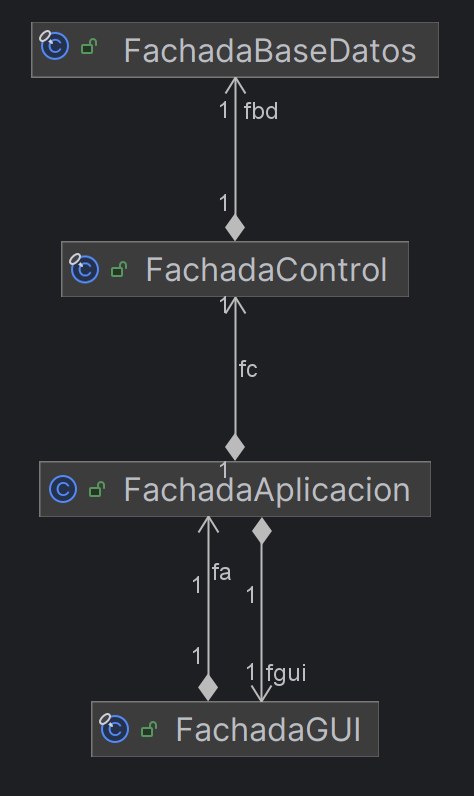
\includegraphics[width=0.59 \linewidth,keepaspectratio]{imagenes/bicifast}
    \caption[Diagrama de arquitectura]{Diagrama de arquitectura por capas}
    \label{fig:diagrama_arquitectura_simple_paquetes}
\end{figure}

\subsection{Componentes identificados y sus responsabilidades}\label{subsec:componentes-identificados-y-sus-responsabilidades}
Después de hacer un análisis de los requisitos funcionales y no funcionales,
hemos definido los siguientes componentes y sus responsabilidades:

\subsubsection{Componentes identificados}
\begin{itemize}
    \item \textbf{Formularios de la GUI:} Son los responsables de la interacción con el usuario y de la presentación de la información.
    \item \textbf{Controladores (Servicios y lógica de negocio):} Gestionan la lógica de la aplicación e interceden entre los DAO y la interfaz gráfica.
    \item \textbf{DAO:} Se encargan de «hablar» con la base de datos.
    Permiten encapsular y abstraer la base de datos y a los datos mismos de la lógica de la aplicación.
    \item \textbf{Base de datos:} Gestiona los datos «permanentes».
\end{itemize}

\subsubsection{Responsabilidades}
Para cada componente, hemos identificado las siguientes responsabilidades funcionales:
\begin{description}
    \item[\textbf{GUI (Presentación)}]
    \begin{itemize}
        \item Mostrar la interfaz gráfica.
        \item Gestionar las diferentes vistas.
    \end{itemize}
    \item[\textbf{Controladores (Servicios)}]
    \begin{itemize}
        \item Gestionar usuarios.
        \item Autentificar.
        \item Cambiar datos.
        \item Gestionar alquileres.
        \item Gestionar la criptografía.
    \end{itemize}
    \item[\textbf{DAOs (Data Access Object)}]
    \begin{itemize}
        \item Hacer consultas a la base de datos.
        \item Modificar la base de datos.
        \item Eliminar entradas de la base de datos.
    \end{itemize}
    \item[\textbf{Base de datos (Persistencia)}]
    \begin{itemize}
        \item Guardar los datos de:
        \begin{itemize}
            \item Usuarios
            \item Bicicletas
            \item Estaciones
            \item Alquileres
        \end{itemize}
    \end{itemize}
\end{description}

\subsection{Dependencias y flujos de control}\label{subsec:dependencias-y-flujos-de-control}
El flujo habitual de control de la aplicación es el que se muestra en la \autoref{fig:flujo_control}.
\begin{figure}[hbpt]
    \centering
    \fbox
    {
        \( \text{[GUI]} \rightarrow \text{[FachadaAplicacion]} \rightarrow \text{[FachadaControl]} \rightarrow \text{[Gestores / BD]} \)
    }
    \caption[Flujo de control]{Flujo de control}
    \label{fig:flujo_control}
\end{figure}
En este flujo, la \textit{GUI} envía una petición a la \textit{FachadaAplicacion}, que delega en la \textit{FachadaControl} para que gestione la petición y
pueda solicitar a la \textit{FachadaBaseDatos} el acceso/almacenamiento de datos en la base de datos.

Ciertamente, existen algunas dependencias cíclicas entre las clases de la capa de presentación, la fachada de presentación
y la fachada de aplicación, ya que la \textit{FachadaAplicacion} necesita conocer la \textit{FachadaGUI} para poder enviarle mensajes.
Puede parecer alarmante, pero no es un problema, ya que el ciclo ocurre principalmente dentro de la capa de presentación y no afecta a la lógica de negocio.
Además, las llamadas desde la \textit{FachadaAplicacion} a la \textit{FachadaGUI} son para situaciones muy específicas, como cambiar el idioma o relanzar la interfaz.

\subsection{Rationale de la arquitectura}\label{subsec:justificacion-de-la-arquitectura}
La elección de la arquitectura por capas se ha tomado por su capacidad de desacoplar y diferencias las responsabilidades de las distintas capas.
Gracias a esta arquitectura, este sistema gana mayor facilidad de mantenimiento, escalabilidad y modularidad.


Por otro lado, la elección del patrón \textit{Façade} se ha tomado por su capacidad de simplificar la interfaz de las capas y facilitar la comunicación entre ellas.
Este patrón permite ocultar la complejidad de las capas y proporcionar una interfaz más sencilla y fácil de usar.
El otro patrón utilizado es el \textit{DAO}, que centraliza y separa el acceso a datos en módulos específicos.
Evitando malas prácticas como el acceso directo a la base de datos desde la capa de presentación o la capa de negocio.